\documentclass[12pt,a4paper]{article}
\usepackage[in]{fullpage}
\usepackage[utf8x]{inputenc}
\usepackage{cite}
%\usepackage{listings}
\usepackage[usenames]{xcolor}
\usepackage{graphicx}
\usepackage{hyperref}
\usepackage{xr} % cross-reference across files
%\usepackage{dirtree} % make directory tree
\usepackage{float} %for H positioning

\externaldocument[TUT-]{tutorial}

% start a new section on a new page
\let\stdsection\section
\renewcommand\section{\newpage\stdsection}

%\lstset{ %
%  basicstyle=\footnotesize,        % the size of the fonts that are used for the code
%  breakatwhitespace=true,          % sets if automatic breaks should only happen at whitespace
%  breaklines=true,                 % sets automatic line breaking
%  commentstyle=\color{gray},    % comment style
%  keepspaces=true,                 % keeps spaces in text, useful for keeping indentation of code (possibly needs columns=flexible)
%  language=bash                 % the language of the code
%}

%opening
\title{EVR Manual}
%\author{Sašo Skube, PSI}

\begin{document}

\maketitle

%\begin{abstract}
%\end{abstract}

\tableofcontents

%\newpage

\section{Introduction}\label{sec:Introduction}
Event receiver is a part of a timing system. A timing system consists of an event generator (EVG), a series of event receivers (EVR), software controlling them and a timing network. EVG generates a series of events, which are delivered to EVRs through a timing network. An EVR is then configured to respond to specific events in various ways, including processing EPICS records and generating pulses, synchronized clock or custom signals on its outputs.

mrfioc2~\cite{mrfioc2} is an EPICS module for the Micro Research Finland(MRF)~\cite{mrf} timing system. The module enables us to configure and use the event generators and event receivers in the timing system. It comprises of EPICS device support for MRF timing system and devlib2 with additional kernel modules (eg. PCIe) for communication with the hardware.

The rest of this document describes the mrfioc2 module in regards to the Event Receiver. EVR and its configuration is described, then instructions for starting a new IOC application are provided. The document continues with basic developer information for the mrfioc2 module and ends with a short description of the EVR GUI. Some sections deal with PSI specifics. These are mostly simplifications in the deployment or build process for the mrfioc2 module.

\section{Event Receiver}\label{sec:Event Receiver}
EVRs are available in various form factors, each supporting the same basic functionality (executing functions, manipulating DBus,...), but with different number of components (inputs, outputs,...). Each of the EVR components and functionalities is configurable by the user and is briefly described in the following sections. It is possible to configure the EVR through the GUI~\ref{sec:GUI} at runtime, or by setting the appropriate macros in the substitution file\footnote{On the PSI infrastructure, a prepared substitution file for VME-EVR-230RF form factor \texttt{mrfioc2/PSI/evr\_ex.subs} with all the macros and short documentation is available (file list item~\ref{itm:files:evr_substitution} in Section~\ref{sec:PSI specifics})} of your IOC application.

%The EVR and its components are configured by setting macros in a form factor specific substitution file. A prepared substitution file for VME-EVR-230RF form factor (file list item~\ref{itm:files:evr_substitution}) is available at~\cite{substitution_git}. All the macros are already present in the substitution file and set to their default values, so the user can simply change the desired values. The substitution file also contains short documentation next to the macros. It is also possible to configure the EVR through the GUI at runtime.

%Each of the EVR components is configurable by the user and is briefly described in the following sections. The available macros are listed using their name and default value. Where many components with the same settings are available (eg. many pulsers), the macro names will reflect the first component (eg. pulser 0).

\paragraph{How to read this section:}
Each sub-section starts with a short description of an EVR component or functionality. It is followed by the description of available macros, that can be used in a substitution file to configure the specific component or functionality of the EVR.
Macro name, its default value, a description, available settings with values or other important information regarding the configuration is listed.
\begin{quote}
Example: \textbf{macro name}=\emph{default value} : Description, with available settings. \texttt{Setting name (macro value)} or \texttt{important information} is emphasized.
\end{quote}
The exact number of form factor specific components is available in~\cite{mrm_evr}. 
%Where there is a number of components with the same settings available(eg. 16 pulsers), only macros for the first component are described(eg. pulser 0).

%An example system name ``MTEST-VME-EVRTEST'' is used. You should change it to fit your application.

%\paragraph{The VME-EVR-230RF form factor} has the following component support:
%\begin{itemize}
%  \item 16 Pulse Generators, named Pul0 - Pul15. Pul0 - Pul3 have additional prescalers.
%  \item 3 Prescalers, named PS0 - PS2
%  \item 2 Front Panel TTL inputs, named FPIn0 - FPIn1
%  \item 4 Front Panel TTL Outputs, named FrontOut0 - FrontOut3
%  \item 3 Front Panel CML Outputs, named FrontOut4 - FrontOut6
%  \item 4 Front Panel Universal I/O in two slots. FrontUnivOut0 and FrontUnivOut1 belong to slot 0, where FrontUnivOut2 and FrontUnivOut3 belong to slot 1. Each slot has 4 additional GPIO pins.
%  \item 16 Rear universal outputs, named RearUniv0 - RearUniv15
%\end{itemize}

\subsection{General configuration}
Each event receiver must be given a name, and belongs to a system. There is additional configuration option for form factors supporting GTX outputs (more about these is available in~\cite{mrm_evr}).

\paragraph{Substitution file macros}
\begin{itemize}
\item
	\textbf{SYS}=\emph{MTEST-VME-EVRTEST} : The system name. 
\item
	\textbf{EVR}=\emph{EVR0} : The name of the connected Event Receiver, which should be the same as defined in the startup script. 
\item
	\textbf{ExtInhib-Sel}=\emph{0} : This macro takes effect only when
configuring GTX ouputs on cPCI-EVRTG-300 form factor. Either honor
the hardware inhibit signal(\texttt{0}) or don't care about hardware
inhibit input state(\texttt{1}). More information is available in~\cite{mrm_evr}.
\end{itemize}

\subsection{Distributed Bus (DBus)}\label{sec:DBus}
The distributed bus is able to carry 8 signals, that are propagated throughout the timing network with the event clock rate. Individual DBus signals (bits) can be outputted through programmable outputs(FrontOut, FrontUnivOut, RearUniv). 

\subsection{Events and event clock}\label{sec:Events and event clock}
EVR receives events transmitted by an event generator from the timing network. Event clock is the frequency, at which the events are received. All the EVRs lock to the phase and frequency of the EVG, thus the event clock is synchronized across the entire timing system.

\paragraph{Substitution file macros}
\begin{itemize}
\item
	\textbf{Link-Clk-SP}=\emph{124.916} : The event receiver requires a
reference clock to be able to synchronize on the incoming event
stream sent by the event generator. For flexibility, a programmable
reference clock is provided to allow the use of the equipment in
various applications with varying frequency requirements. It must be
close enough to the EVG clock to allow phase locking with
EVR. Available values are \texttt{50 MHz - 150 MHz}. 
%The clock reference for the event receiver is generated on-board the event receiver using a fractional synthesizer.
\item
\textbf{Link-RxMode-Sel}=\emph{1} : Set whether the \texttt{DBus(0)} or
\texttt{DBus + Data Buffer(1)} are sent downstream (to the timing network). Distributed bus bandwidth may be shared by transmission of a configurable size data buffer to up to 2 kbytes. When data transmission is enabled the distributed bus bandwidth is halved. 
\end{itemize}


\subsection{Pulse Generator - Pulser (Pul)}\label{sec:Pulser}
A pulse generator is able to output a configured pulse upon reception of an event.
\begin{figure}[H]
	\centering
	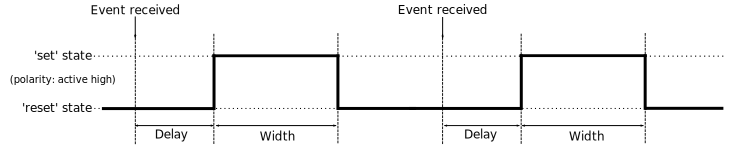
\includegraphics[width=\columnwidth]{./img/pulserGeneric}
	\caption{An example of 2 pulses generated after the reception of the event.}
	\label{fig:pulser_generic}
\end{figure}
Figure~\ref{fig:pulser_generic} shows how the pulse is generated by switching between set and reset states, where the states determine the logic level of the pulser output signal.

The pulser has configurable properties:
\begin{itemize}
	\item \textbf{Polarity} determines the logic level of the \texttt{set} and \texttt{reset} states. When polarity is set to
	\begin{itemize}
		\item \texttt{active high}, the \texttt{set state} puts the pulser output to logic high and the \texttt{reset state} puts the pulser output to logic low. 
		\item \texttt{active low}, the \texttt{set state} puts the pulser output to logic low and the \texttt{reset state} puts the pulser output to logic high.
	\end{itemize}
	\item  \textbf{Delay} determines the time from when the event was received to when the pulser enters the \textit{set state}.
	\item  \textbf{Width} determines the time from when the pulser enters the \textit{set state} to when it enters the \textit{reset state}.
\end{itemize}

\paragraph{Substitution file macros}
There are a maximum of 16 pulsers available, depending on the EVR form factor. Pulsers are named Pul\#, where \# is the ID of the pulser ranging, from 0 to 15.
\begin{itemize}
  \item
    \textbf{Pul\#-Ena-Sel}=\emph{1} When \texttt{disabled(0)}, the output
    of the pulser will remain in its reset state. The pulser must be
    \texttt{enabled(1)} when used.
  \item
    \textbf{Pul\#-Polarity-Sel}=\emph{0} : Sets the pulser \textbf{polarity} to \texttt{active high(0)} or \texttt{active low(1)}.
  \item
    \textbf{Pul\#-Delay-SP}=\emph{0} : Sets the pulse \textbf{delay} in range of \texttt{0 us - 4294967295 us}.
  \item
    \textbf{Pul\#-Width-SP}=\emph{0} : Sets the pulse \textbf{width} in range of \texttt{0 us- 65535 us}.
  \item
    \textbf{Pul\#-Prescaler-SP}=\emph{1} : Decreases the resolution of
    both \textbf{delay} and \textbf{width} by an integer factor. Value range:
    \texttt{0-255}. Pulsers without prescalers use a fixed prescale
    value of 1.
  \end{itemize}

Each received event can activate a function of the pulser:
\begin{itemize}
	\item \textbf{Trig} function uses polarity, delay and width to generate a pulse. Pulser starts in \texttt{reset state}. After the reception of an event, pulser waits \texttt{delay} ns and goes to \texttt{set state}. Then it waits for \texttt{width} ns and goes back to \texttt{reset state}.
	\item \textbf{Set} function puts the pulser to \texttt{set state}. Delay and width properties are ignored.
	\item \textbf{Reset} function puts the pulser to the \texttt{reset state}. Delay and width properties are ignored.
\end{itemize}

\textbf{Substitution file macros} for mapping events to pulser function are available in Section~\ref{sec:Pulser mapping}, together with an \textbf{example}.

\subsection{Prescaler (PS)}\label{sec:Prescaler}
Prescalers can be configured to output the event clock divided by an integer factor. There is a special event 123 (0x7b) that resets all the prescalers, so that the prescaled signal is in the same phase across all EVRs.

\paragraph{Substitution file macros}
There are a maximum of 4 prescalers available, depending on the EVR form factor. Prescalers are named PS\#, where \# is the ID of the prescaler, ranging from 0 to 3.
\begin{itemize}
  \item
    \textbf{PS\#-Div-SP}=\emph{2} : Sets the integer divisor between the
    event clock and the prescaled event clock output in a range of
    \texttt{2-65535}.
  \end{itemize}


\subsection{Front Panel TTL Input (FPIn)}\label{sec:Front Panel TTL Input}
Front panel inputs can also be called External Event Inputs, because they can be configured to cause an event. The event can be local to the EVR (trigger mode) or sent through the timing network (backwards mode) when a condition occurs. The conditions are configured to respond to the front panel input signal logic level (level condition) or input signal edge (edge condition). Events generated by the front panel input logic are handled as any other events. Front panel inputs also provide configuration options for DBus signal manipulation.

\paragraph{Substitution file macros}
There are a maximum of 2 front panel TTL inputs available, depending on the EVR form factor. Front panel TTL inputs are named FPIn\#, where \# is the ID of the front panel TTL input, ranging from 0 to 1.
\begin{itemize}
  \item
    \textbf{FPIn\#-Lvl-Sel}=\emph{1} : Determines if event is sent when the input signal logic level is low \texttt{Active Low(0)} or high \texttt{Active High(1)}, when using the \texttt{level} condition.
  \item
    \textbf{FPIn\#-Edge-Sel}=\emph{1} : Determines if event is sent on the falling \texttt{Active Falling(0)} or rising \texttt{Active Rising(1)} edge of the input signal, when using the \texttt{edge} condition.
  \item
    \textbf{FPIn\#-Trig-Ext-Sel}=\emph{0} : Selects the condition (\texttt{Off(0)}, \texttt{Level(1)} or \texttt{Edge(2)}) on which to trigger an event local to the EVR. This is the trigger mode condition.
  \item
    \textbf{FPIn\#-Code-Ext-SP}=\emph{0} : Sets the event which will be sent to timing network, whenever the trigger mode condition is met. Any event in range of \texttt{0-255} can be selected.
  \item
    \textbf{FPIn\#-Trig-Back-Sel}=\emph{0} : Selects the condition (\texttt{Off(0)}, \texttt{Level(1)} or \texttt{Edge(2)}) in which to send an event to the timing network. This is the backward mode condition.
  \item
    \textbf{FPIn\#-Code-Back-SP}=\emph{0} : Sets the event which will be sent to timing network, whenever the backwards mode condition is met. Any event in range of \texttt{0-255} can be selected.
  \item
    \textbf{FPIn\#-DBus-Sel}=\emph{0} : Set the upstream DBus bit mask which is driven by this input. DBus bits and the macro value are condensed with a bit-wise OR. Available values for the DBus bit mask are: \texttt{1 = Bit 0, 2 = Bit 1, 4 = Bit 2, 8 = Bit 3, 16 = Bit 4, 32 = Bit 5, 64 = Bit 6, 128 = Bit 7}.
  \end{itemize}
  
  
\subsection{Outputs}\label{sec:Outputs}
\begin{figure}[H]
	\centering
	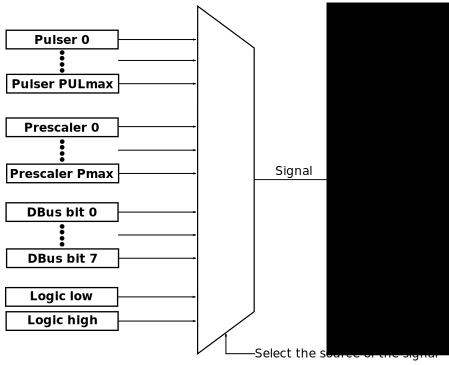
\includegraphics[]{./img/output}
	\caption{Available source signals for each output}
	\label{fig:output}
\end{figure}

An EVR has a number of outputs, each with a configurable source signal. As seen in Figure~\ref{fig:output}, any of the available pulser, prescaler, DBus, logic low or logic high signals can be selected as the output source signal. Depending on the output type(TTL, CML, ...), the signal can be outputted directly, further manipulated or used as a trigger for a special function of that output.

\paragraph{Substitution file macros common to all outputs:} Outputs, and the corresponding macro name prefixes, are named either \emph{FrontOut\#},\emph{ FrontOutUniv\#} or \emph{RearUniv\#}, where the range of the number \# depends on the EVR form factor. Macros for the \emph{FrontOut0} are described below. 
%The source of the output signal is determined by mappings in Table~\ref{tab:mappings}. 

\begin{table}[!hbt]
\caption{Output source signal mappings}
\label{tab:mappings}
\centering
	\begin{tabular}{|c|c|}
		\hline \textbf{mapping} & \textbf{output source} \\ \hline 
		\hline 0 & Pulser 0 \\ 
		\hline 1 & Pulser 1 \\ 
		\hline 2 & Pulser 2 \\ 
		\hline 3 & Pulser 3 \\ 
		\hline 4 & Pulser 4 \\ 
		\hline 5 & Pulser 5 \\ 
		\hline 6 & Pulser 6 \\ 
		\hline 7 & Pulser 7 \\ 
		\hline 8 & Pulser 8 \\ 
		\hline 9 & Pulser 9 \\ 
		\hline 10 & Pulser 10 \\ 
		\hline 11 & Pulser 11 \\ 
		\hline 12 & Pulser 12 \\ 
		\hline 13 & Pulser 13 \\ 
		\hline 14 & Pulser 14 \\ 
		\hline 15 & Pulser 15 \\ 
		\hline 32 & Distributed bus bit 0 \\ 
		\hline 33 & Distributed bus bit 1 \\ 
		\hline 34 & Distributed bus bit 2 \\ 
		\hline 35 & Distributed bus bit 3 \\ 
		\hline 36 & Distributed bus bit 4 \\ 
		\hline 37 & Distributed bus bit 5 \\ 
		\hline 38 & Distributed bus bit 6 \\ 
		\hline 39 & Distributed bus bit 7 \\ 
		\hline 40 & Prescaler 0 \\ 
		\hline 41 & Prescaler 1 \\ 
		\hline 42 & Prescaler 2 \\ 
		\hline 62 & Logic High \\ 
		\hline 63 & Logic low \\ 
		\hline 
	\end{tabular} 
\end{table}

  \begin{itemize}
  \item
   \textbf{FrontOut0-Ena-SP}=\emph{1} : When set to \texttt{enabled(1)} the mapping
    defined in \newline \texttt{FrontOut0-Src-SP} is used. When \texttt{disabled(0)}, a
    mapping of \texttt{Force Low(63)} from Table~\ref{tab:mappings} is used.
  \item
    \textbf{FrontOut0-Src-SP}=\emph{63} : \texttt{Mappings} from the Table~\ref{tab:mappings} are
    set here. Any of the available pulser, prescaler, DBus, logic low or
    logic high signals can be selected as the output source signal.
  \end{itemize}

\subsubsection{Front Panel TTL Output (FrontOut)}\label{sec:Front Panel TTL Output}
These outputs are capable of driving TTL compatible logic level signals. The output source signal is converted to TTL logic levels(LVTTL of max 3.3 Volts) and outputted, as seen in Figure~\ref{fig:output_ttl}.

\begin{figure}[H]
	\centering
	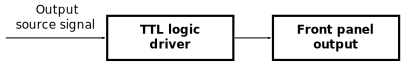
\includegraphics[]{./img/TTL}
	\caption{Front panel TTL output}
	\label{fig:output_ttl}
\end{figure}

\subsubsection{Front Panel CML Output (FrontOut)}\label{sec:Front Panel CML Output}
These outputs are capable of driving Current-mode logic compatible signals. Based on the output source signal and the selected CML mode, various patterns can be outputted. As seen in Figure~\ref{fig:output_cml}, patterns are generated using one of the three configurable modes. They are sent out at 20 times the bit rate of the event clock, thus the outputs allow for producing fine grained adjustable pulses and clock frequencies. 	
\begin{figure}[H]
	\centering
	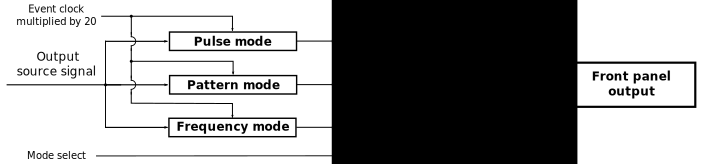
\includegraphics[width=\columnwidth]{./img/CML}
	\caption{Overview of the front panel CML outputs}
	\label{fig:output_cml}
\end{figure}

\paragraph{Substitution file macros} for general CML configuration:
There are a maximum of 8 CML outputs available, depending on the EVR form factor. CML outputs are named CML\#, where \# is the ID of the CML output, ranging from 0 to 7. Some form factors do not have any CML outputs.
\begin{itemize}
\item
  \textbf{CML0-Ena-Sel}= \emph{0} : Output is \texttt{disabled(0)} or \texttt{enabled(1)}.
\item
  \textbf{CML0-Pwr-Sel}=\emph{0} : Outputs can be \texttt{powered down(0)} or in normal \texttt{operation(1)}.
\item
  \textbf{CML0-Rst-Sel}=\emph{0} : It is possible to \texttt{reset CML output(1)} or leave it in \texttt{normal operation(0)}.
\item
  \textbf{CML0-Mode-Sel}=\emph{0} : There are three configurable modes, \texttt{pattern mode(0)}, \texttt{frequency mode(1)} and \texttt{waveform mode(2)}.
\end{itemize}
Patterns are defined by one of the configurable CML modes:
\begin{itemize}
\item 
	In \textbf{pulse mode}, the output logic monitors, and distinguishes between the states of the output source signal(logic low, rising edge, logic high, falling edge). Based on this state, a user configurable 20-bit pattern is sent out.
	
	\paragraph{Patterns configurable through the GUI:}
	\begin{itemize}
	\item
	  signal is \textbf{rising}: pattern is sent out
	  after the rising edge is detected and will interrupt the current
	  pattern being sent.
	\item
	  signal is \textbf{falling}: pattern is sent out
	  after the falling edge is detected and will interrupt the current
	  pattern being sent.
	\item
	  signal is \textbf{high}: pattern is sent out after
	  the rising edge is detected and will repeat until the falling edge.
	\item
	  signal is \textbf{low}: pattern is sent out after
	  the falling edge is detected and will repeat until the rising edge.
	\end{itemize}
\item 
	In \textbf{frequency mode}, clocks with clock period in steps of 1/20 of the event clock period can be generated. The clock output is synchronized by the output source signal(pulser, DBus signal, ....). 
	
	This frequency generator is triggered by a rising edge of the output source signal. After the trigger, it waits for a configured initial delay before it starts to generate a clock signal. 
%	The signal is generated by switching between set and reset states. The states determine the logic level of the frequency generator output signal.
		
	\paragraph{Substitution file macros}
	\begin{itemize}
	\item
	  \textbf{CML0-Freq:Lvl-SP}=\emph{0} : set the starting logic level of the frequency generator. Options are:
	  \begin{itemize}
	  	\item \texttt{Active high(0)}: starting logic level is logic high
	  	\item \texttt{Active low(1)}: starting logic level is logic low
	  \end{itemize}
	\item
	  \textbf{CML0-Freq:Init-SP}=\emph{0} : Set the initial delay between when the frequency generator is triggered and when it starts to generate a clock signal. This allows for a phase difference between the output source signal and the output signal. The value range in ns depends on the event clock. It must be in range of 1 event clock period to 3276 event clock periods.
	\item
	  \textbf{CML0-Freq:High-SP}=\emph{10} : sets the amount of time in ns the signal stays on logic high, before switching to logic low. The value range in ns depends on the event clock. It must be in range of $20/20=1$ event clock period to $65536/20$ event clock periods.
	\item
	  \textbf{CML0-Freq:Low-SP}=\emph{10} : sets the amount of time in ns the signal stays logic low, before switching to logic high. The value range in ns depends on the event clock. It must be in range of $20/20=1$ event clock period to $65536/20$ event clock periods.
	\end{itemize}
\item 
	In \textbf{pattern mode}, one can generate arbitrary bit patterns(waveforms), triggered by the output source signal(pulser, DBus signal,...). The waveform length is in multiple of 20 bits (each bit is 1/20 of the event clock period), where maximum waveform length is 20x2048 bits.
	%	  \textbf{timeline} (\emph{Pat:WfX-I}): displays the times at which an  element from the pattern will be sent out.
		
	\paragraph{Substitution file macros}
	\begin{itemize}
	\item
	  \textbf{CML0-Pat:WfCycle-SP}=\emph{0} : In \texttt{single shot mode(0)} the
	  waveform is sent only once per received trigger, where in \texttt{loop mode(1)}
	  the pattern will continuously loop after the first trigger occurred.
	\end{itemize}
	
	There are two additional calculators available to simplify waveform creation. 
	\paragraph{A delay calculator} has configurable \texttt{delay} and \texttt{width} macros to generate a pulse(similar to a pulser):
	\begin{itemize}
	\item
	  \textbf{CML0-WfCalc:Ena-SP}=\emph{0} : \texttt{enable(1)} or \texttt{disable(0)} the calculation.
	\item
	  \textbf{CML0-WfCalc:Delay-SP}=\emph{16} : can be used to specify the time in ns between when the mode is triggered and the pulse is generated. The value range in ns depends on the event clock. It must be in range of 1 event clock period to 2048 event clock periods.
	\item
	  \textbf{CML0-WfCalc:Width-SP}=\emph{50} : can be used to specify the width of the pulse - the time the signal is stable at logic high. The value range in ns depends on the event clock. It must be in range of 1 event clock period to 2048 event clock periods.
	\end{itemize}
	
	\paragraph{A bunch train calculator} that generates a series of consecutive pulses with width and delay fixed to $(event clock) / 4$. As seen in Figure~\ref{fig:output_cml_bunch}, each bunch pattern consists of 5 logic low bits and 5 logic high bits. A bunch train always ends with 10 logic low bits.
	\begin{figure}[H]
		\centering
		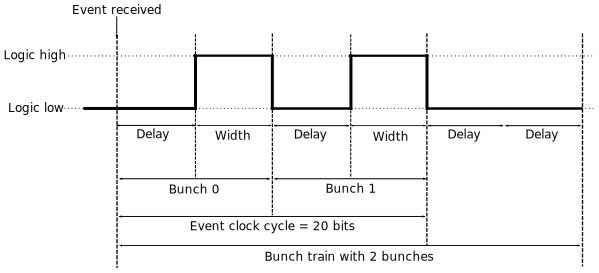
\includegraphics[width=0.96\columnwidth]{./img/bunchTrain}
		\caption{A bunch train example with 2 bunches}
		\label{fig:output_cml_bunch}
	\end{figure}
	
	Bunch train calculator has the following substitution macros for configuration:
	\begin{itemize}
	\item
	  \textbf{CML0-BunchTrain:Ena-SP}=\emph{0} : \texttt{enable(1)} or \texttt{disable(0)} the bunch train calculator
	\item
	  \textbf{CML0-BunchTrain:Size-SP}=\emph{1} : set the number of bunches per train in range of \texttt{1-150}.
	\end{itemize}
	
\end{itemize}


\subsubsection{Front Panel Universal I/O (FrontUnivOut)}\label{sec:Front Panel Universal I/O}
Universal I/O slots provide different types of input or output with exchangeable Universal I/O modules~\cite{mrf}. Each module provides two inputs or outputs (TTL, NIM or optical). 
The exact output signal is dependent on the inserted module. Figure~\ref{fig:output_univ}, shows an example of a universal I/O module with two outputs inserted in front panel universal slot.
\begin{figure}[H]
	\centering
	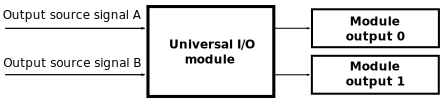
\includegraphics[]{./img/univ}
	\caption{An example universal I/O module with two outputs.}
	\label{fig:output_univ}
\end{figure}

\subsubsection{Rear Universal output - Transition Board output (RearUniv)}\label{sec:Rear Universal output}
An EVR has additional rear universal outputs. They are located on the back-plane of the EVR board. The exact output signal is dependent on the universal module inserted in the transition board.

\subsection{Time stamping mechanism}\label{sec:Time stamping mechanism}
\begin{quote}
\textbf{The functionality of the time stamping mechanism was not tested!}
\end{quote}
The event receiver supports a global time stamping mechanism. Time-stamp consists of a 32-bit time-stamp event counter and a 32-bit seconds counter. The seconds counter can be updated from the
shift register. Counters are clocked using prescaled event clock, DBus bit 4, or on each reception of the mapped event (\texttt{TS Tick} special function described in Section~\ref{sec:Special functions}). If configured, events together with their time-stamp are stored in a FIFO memory.

\begin{itemize}
\item
	\textbf{Time-Src-Sel}=\emph{0} : Determines what causes the
timestamp event counter to increment.

\begin{itemize}
\item
  The \texttt{event clock(0)} source will use a prescaled EVR
  reference clock.
\item
  The \texttt{mapped codes(1)} increment the counter whenever
  certain event arrives. Time-stamp counter event can be defined using a \texttt{TS Tick} special function described in Section~\ref{sec:Special functions}.
\item
  \texttt{DBus bit 4(2)} will increment the counter on the
  low-to-high transition of the DBus bit 4.
\end{itemize}
\item
	\textbf{Time-Clock-SP}=\emph{0.0} : Specifies the rate at which the
timestamp event counter will be incremented. This determines the
resolution of all timestamps. Use \textbf{in conjunction with} the \texttt{Time-Src-Sel}.

When the timestamp source(\texttt{Time-Src-Sel}) is set to \texttt{Event clock}
this macro value is used to prescale the EVR's reference clock
frequency to the given frequency. Since this may not be exact it is
recommended to read back the actual divider setting via the
timestamp prescaler (\texttt{\$(SYS)-\$(EVR):Time-Div-I} record). In
all modes this value is stored in memory and used to convert the
timestamp event counter values from ticks to seconds. The units are
in \texttt{MHz}.
\end{itemize}

\subsection{Heartbeat monitor}\label{sec:Heartbeat monitor}
A heartbeat monitor is provided to receive heartbeat events from the timing network. If no heartbeat event is received (in approx. 1.6 s), the heartbeat timeout occurs and a heartbeat flag is set. 
%The event receiver may be programmed to generate a heartbeat interrupt.

\subsection{Delay module}\label{evr-delaymodule.template}
EVR has universal I/O slots, described in Section~\ref{sec:Front Panel Universal I/O}, where universal modules can be inserted. One of these is UNIV-LVPECL-DLY Delay module. This module will output a delayed signal from the appropriate FrontUnivOut output. The FrontUnivOut output source signal can be configured as described in Section~\ref{sec:Outputs} using mappings from Table~\ref{tab:mappings}. The delay can be configured from 2200 ps to 12430 ps, with 10 ps resolution. 

%Using the inserted module with the prepared substitution file(file list item~\ref{itm:files:evr_substitution} in Section~\ref{sec:PSI specifics}) is simple. User only needs to uncomment the substitution definition and macros for the appropriate slot.

\paragraph{Substitution file macros}
\begin{itemize}
\item
	\textbf{SYS}=\emph{MTEST-VME-EVRTEST} : The system name.
\item
	\textbf{EVR}=\emph{EVR0} : The name of the event receiver, where the module is inserted.
\item
  \textbf{SLOT} : The universal slot of the EVR, where the module is inserted. FrontUnivOut0 is the first and FrontUnivOut1 is the second output of slot \texttt{0}, where FrontUnivOut2 is the first and FrontUnivOut3 is the second output of slot \texttt{1}.
\item
  \textbf{Enabled}=\emph{1} : \texttt{enable(1)} or \texttt{disable(0)} the module.
  When disabled, both outputs are pulled to logic low.
\item
  \textbf{Delay0}=\emph{2.2} : is a tunable delay for the first output. The value is
  in range of \texttt{2.2 ns - 12.43 ns}.
\item
  \textbf{Delay1}=\emph{2.2} : is a tunable delay for the second output. The value
  is in range of \texttt{2.2 ns - 12.43 ns}.
\end{itemize}

\paragraph{Example:} Both front panel universal slots of the EVR0 are occupied since there are
two delay modules inserted, one in slot 0 and one in slot 1. Module in
slot 0 is enabled and has first output set to minimum delay and second
output to maximum delay. Module in slot 1 is disabled with both output
delays set to 5ns. The EVR belongs to the MTEST-VME-EVRTEST system.

\begin{verbatim}
file "evr-delayModule.template"
{
    { SYS     = MTEST-VME-EVRTEST,
      EVR     = EVR0,
      SLOT    = 0,

      Enabled = 1,
      Delay0  = 2.20,
      Delay1  = 12.43,
    }
    { SYS     = MTEST-VME-EVRTEST,
      EVR     = EVR0,
      SLOT    = 1,

      Enabled = 0,
      Delay0  = 5,
      Delay1  = 5,
    }
}
\end{verbatim}

\subsection{Event mapping}\label{sec:Event mapping}
As mentioned in Section~\ref{sec:Introduction}, an EVR responds to events. In order for the EVR to respond, an appropriate mapping between the event and  EVR function/component needs to be configured.

%an appropriate mapping needs to be configured. 

%to trigger an EVR action or a EVR component an appropriate mapping between the event and action/component needs to be configured. When an appropriate mapping is configured, received event triggers the mapped EVR component or action. 

\subsubsection{Trigger an EPICS event}\label{evr-softevent.template}
Provide us with the ability to map between EPICS event (software) and an event from the timing system (hardware).

\paragraph{Substitution file macros:}
\begin{itemize}
	\item
		\textbf{SYS}=\emph{MTEST-VME-EVRTEST} : The system name.
	\item
		\textbf{EVR}=\emph{EVR0} : The name of the connected Event Receiver, which should be the same as defined in the startup script. 
	\item
	  \textbf{EVT} represents the event from the timing system. Set EVT=0 to disable.
	\item
	  \textbf{CODE} represents EPICS event number (software).
\end{itemize}

\paragraph{Example:} The configuration applies to EVR0 in the MTEST-VME-EVRTEST system. EPICS event 1 is set to trigger when an event 1 from the timing system is received, and EPICS event 2 to trigger on reception of event 2 from the timing system. It is \texttt{recommended to use the same EPICS event and timing system event numbers}, but it is not mandatory.

\begin{verbatim}
file "evr-softEvent.template"{
pattern { SYS,                   EVR,    EVT,    CODE}
        {"MTEST-VME-EVRTEST",   "EVR0",  "1",    "1"}
        {"MTEST-VME-EVRTEST",   "EVR0",  "2",    "2"}
}
\end{verbatim}

It is also possible to manually forward link an appropriate event record instead of using EPICS events. The functionality of EPIC events and links is out of the scope of this documents.

\subsubsection{Special functions}\label{sec:Special functions}
There is a number of special functions available, that can be activated
on specified event. Each event can be mapped only to one function. There
exist some default events, that always trigger specific function.

\paragraph{EVR functions:}
\begin{itemize}
\item
  \textbf{Blink} : An LED on the EVRs front panel will blink when the
  event is received.
\item
  \textbf{Forward} : The received event will be immediately retransmitted
  on the upstream event link.
\item
  \textbf{Stop Log} : Freeze the circular event log buffer which contains up to 512 events with time-stamp information. A CPU interrupt will be raised which will cause this buffer to be downloaded. This might be a useful action to map to a fault event. (default event 121)
\item
  \textbf{Log} : Include this event code in the circular event log.
\item
  \textbf{Heartbeat} : This event resets the heartbeat timeout. See Section~\ref{sec:Heartbeat monitor} for details. (default event 122)
\item
  \textbf{Reset PS} : Resets the phase of all prescalers. (default event 123)
\item
  \textbf{TS reset} : Loads the time-stamp seconds counter from the shift register and zeros the time-stamp event counter. See Section~\ref{sec:Time stamping mechanism} for details. (default event 124)
\item
  \textbf{TS tick} : When the time-stamp source is `Mapped code' then any event with this mapping will cause the time-stamp event counter to increment. See Section~\ref{sec:Time stamping mechanism} for details. (default event 125)
\item
  \textbf{Shift 0} : Shifts the current value of the shift register up by one bit and sets the low bit to 0. See Section~\ref{sec:Time stamping mechanism} for details. (default event 112)
\item
  \textbf{Shift 1} : Shifts the current value of the shift register up by one bit and sets the low bit to 1. See Section~\ref{sec:Time stamping mechanism} for details. (default event 113)
\item
  \textbf{FIFO} : Bypass the automatic allocation mechanism and always include this code in the FIFO memory. See Section~\ref{sec:Time stamping mechanism} for details.
\end{itemize}

\paragraph{Substitution file macros:}

\begin{itemize}
\item
	\textbf{SYS}=\emph{MTEST-VME-EVRTEST} : The system name. 
\item
	\textbf{EVR}=\emph{EVR0} : The name of the connected event receiver, which should be the same as defined in the startup script. 
\item
  \textbf{EVT} represents an event from the timing system.
\item
  \textbf{FUNC} represents one of the functions listed above.
\end{itemize}

\textbf{Example}: The following macros configure the event mappings to blink the LED on each occurrence of event 1, and event 6. The configuration applies to EVR0 in the MTEST-VME-EVRTEST system.

\begin{verbatim}
file "evr-specialFunctionMap.template"{
pattern { SYS,                   EVR,    EVT,   FUNC }
        {"MTEST-VME-EVRTEST",   "EVR0",  "1",   "Blink"}
        {"MTEST-VME-EVRTEST",   "EVR0",  "6",   "Blink"}
}
\end{verbatim}

\subsubsection{Pulser mapping}\label{sec:Pulser mapping}
Event receivers have multiple pulsers that can preform several functions upon reception of events (described in Section~\ref{sec:Pulser}). Each pulser-function combination can be
mapped to multiple events.

\paragraph{Substitution file macros:}
\begin{itemize}
\item
	\textbf{SYS}=\emph{MTEST-VME-EVRTEST} : The system name. 
\item
	\textbf{EVR}=\emph{EVR0} : The name of the connected event receiver, which should be the same as defined in the startup script.
\item
  \textbf{PID} represents the pulser number
\item
  \textbf{F} represents one of the functions listed above.
\item
  \textbf{EVT} represents an event from the timing network.
\item
  \textbf{ID} Mappings must have unique ID for each PID-F combination.
%  Only mappings with ID=0 are displayed in the GUI.
\end{itemize}

\paragraph{Example:} Pulser 0 is set to trigger on event 2 and event 3. It will also
reset on event 4. The configuration applies to EVR0 in the MTEST-VME-EVRTEST system.

\begin{verbatim}
file "evr-pulserMap.template"{
pattern { SYS,                   EVR,    PID   F,      EVT, ID }
        {"MTEST-VME-EVRTEST",   "EVR0",  0,    Trig,    2,   0 }
        {"MTEST-VME-EVRTEST",   "EVR0",  0,    Trig,    3,   1 }
        {"MTEST-VME-EVRTEST",   "EVR0",  0,    Reset,   4,   0 }
}
\end{verbatim}


\section{PSI IOC startup}\label{sec:PSI IOC startup}
Section~\ref{TUT-sec:Quick start} of the Tutorial~\cite{tutorial} describes a simple way of using the predefined templates with a generic startup script to create the IOC application. This Section describes how to use the template files directly from the mrfioc2 reporsitory~\cite{git_mrfioc2} with a custom startup script.

The templates are available in \texttt{mrfioc2/evrMrmApp/Db/PSI} folder (folder list item~\ref{itm:folder:evr_db} in Section~\ref{sec:PSI specifics}). The following steps should be taken in order to create a new SWIT compliant IOC application for the Event Receiver:


\begin{enumerate}
%\def\labelenumi{\arabic{enumi}.}
\item
  Create a \textbf{project folder}, eg. \texttt{MTEST-VME-EVRTEST}. Let $ <TOP> $ be the path to this folder, eg $ <TOP> $ = \texttt{\textasciitilde/public/F/TEST/MTEST-VME-EVRTEST}.
\begin{verbatim}
mkdir -p <TOP>
\end{verbatim}
  
\item
  \textbf{Assuming} the form factor is VME-EVR-230RF the template is available at this location: \texttt{mrfioc2/evrMrmApp/Db/PSI/\textbf{evr-vmerf230.template}}. A form factor specific template can also be manually generated as described in Section~\ref{sec:Generating templates}.  

\item
  Copy the template files to your project by issuing the following commands in the \texttt{mrfioc2/evrMrmApp/Db/PSI/} folder:
\begin{verbatim}
cp evr-softEvent.template <top>/
cp evr-pulserMap.template <top>/
cp evr-specialFunctionMap.template <top>/
cp evr-vmerf230.template <top>/
cp evr-delayModule.template <top>/
\end{verbatim}

\item 
  Copy the substitution file to your project by issuing the following commands in the \texttt{mrfioc2/PSI/} folder:
\begin{verbatim}
cp evr_ex.subs <top>/MTEST-VME-EVRTEST_EVR.subs
\end{verbatim}

\item
  Create a \textbf{startup script}
  \texttt{$<TOP>$/MTEST-VME-EVRTEST\_startup.script}, with the following content:

\begin{verbatim}
## Load IFC1210 devLib and pev modules
require 'pev'
## Load mrfioc2 device support
require 'mrfioc2'

##########################
#-----! EVR Setup ------!#
##########################
## Configure EVR
## Arguments:
##  - device name
##  - slot number
##  - A24 base address
##  - IRQ level
##  - IRQ vector

mrmEvrSetupVME(EVR0,2,0x3000000,4,0x28);
var dbTemplateMaxVars 500

## EVR init done
\end{verbatim}

  In this example the EVR named ``EVR0'' is present in VME slot 2. It is
  given a base A24 address of 0x3000000 and configured to interrupt on
  level 4 with interrupt vector 0x28. User should change the parameters of \emph{mrmEvrSetupVME(EVR0, 2, 0x3000000, 4, 0x28);} according to his hardware setup.
  
  \textbf{Unused address range should be selected by the user} based on resources available on VME.
  The user must be confident that the address space is available and free, since the system does not preform any checks. 
  
  However, the system checks if an EVR is available in the selected slot. If it is not found, the EVR setup will abort.
  
  Command \texttt{var dbTemplateMaxVars 500} sets the upper limit for the number of macros processed in the substitution file.
  
\item
  Add \texttt{SYS} and \texttt{EVR} macros and remove \texttt{\$(TEMPLATE\_DIR)/} from each template in the substitution file. SYS is the system name, EVR is the name of the Event Receiver (as defined in the startup script) and \texttt{\$(TEMPLATE\_DIR)/} is the location of the predefined template files. 
  
\paragraph{Example:} 
Original substitution file snippet:

\begin{verbatim}
...
file "$(TEMPLATE_DIR)/evr-softEvent.template"{
pattern { EVT,  CODE }
        { "1",    "1"}
        { "2",    "2"}
        { "3",    "3"}
}
...
\end{verbatim}

 Macros SYS and EVR added and \texttt{\$(TEMPLATE\_DIR)/} removed:

\begin{verbatim}
...
file "evr-softEvent.template"{
pattern { SYS,                  EVR,    EVT,    CODE }
        {"MTEST-VME-EVRTEST",   "EVR0", "1",    "1"}
        {"MTEST-VME-EVRTEST",   "EVR0", "2",    "2"}
        {"MTEST-VME-EVRTEST",   "EVR0", "3",    "3"}
}
...
\end{verbatim}
\item
  Set the macro values in the substitution file according to your needs.
  Detailed description of the macros is available in Section~\ref{sec:Event Receiver}.
  You can also follow the Tutorial~\cite{tutorial} to get acquainted with the EVR basic functions and configuration.
\item
  Optionally, you can remove all the macros whose values you did not
  change.
\item
  \textbf{Install the} prepared \textbf{IOC} by running the command
  \texttt{swit -V} from your project folder $<TOP>$.
\end{enumerate}

\section{Standard IOC startup}
The EPICS way.

\section{mrfioc2 organization}\label{sec:Source code organization}
Some important folders:
\begin{verbatim}
mrfioc2
    |-- configure
    |-- documentation
       |--PSI
    |-- evgMrmApp
        |-- Db
            |-- PSI
        |-- src
    |-- evrApp
        |-- Db
        |-- src
    |-- evrMrmApp
        |-- Db
            |-- PSI
        |-- src
    |-- iocBoot
    |-- mrfCommon
    |-- mrmShared
    |-- mrmtestApp
    |-- PSI
    |-- ui
        |-- EVG
        |-- EVR
\end{verbatim}

\subsection{Source code}
\begin{itemize}
\item 
	\texttt{evgMrmApp/src} contains source files for the an Event Generator.
\item 
	\texttt{evrApp/src} and \texttt{evrmrmApp/src} contains source files for an Event Receiver.
\item 
	\texttt{mrfCommon} contains common functions and definitions used in the mrfioc2 module. 
\item 
	\texttt{mrfShared} contains code shared between EVG and EVR together with some OS specifics.
\item 
	\texttt{/} and \texttt{PSI} contain makefiles for building the mrfioc2 module.
\item 
	\texttt{configure} and \texttt{iocBoot} are standard IOC application folders.
\end{itemize}

\subsection{PSI specifics}\label{sec:PSI specifics}
Some folders:
\begin{enumerate}
\item 
	\texttt{documentation/PSI} contains this document and a tutorial~\cite{tutorial} with step-by-step instructions to configuring some of the basic functionalities of the Event Receiver, including both document sources.
\item 
	\texttt{evgMrmApp/Db/PSI} contains database templates for an Event Generator.\label{itm:folder:evg_db}

\item 
	\texttt{evrMrmApp/Db/PSI} contains database templates for an Event Receiver.\label{itm:folder:evr_db}

\item 
	\texttt{PSI} contains substitution files used in creation of an IOC application and a makefile to build the mrfioc2 module using driver.makefile.\label{itm:folder:psi}
\item 
	\texttt{ui} contains caQtDM screens for Event Receiver and Event Generator in \texttt{EVR} and \texttt{EVG} sub-folder, respectively.
\end{enumerate}
Some files:
\begin{enumerate}
\item 
	\texttt{mrfioc2/evgMrmApp/Db/PSI/evg-vme.template} is an EVG form factor specific template file.\label{itm:files:evg_template}
\item 
	\texttt{mrfioc2/evgMrmApp/Db/PSI/evg-vme.substitutions} is an EVG form factor specific substitution file used to generate the form factor specific template file(list item~\ref{itm:files:evg_template}).\label{itm:files:evg_ff_subs}
\item 
	\texttt{mrfioc2/PSI/evg\_ex.subs} is the EVG substitution used in creation of an IOC application. It contains form factor specific macros for setting up EVG.\label{itm:files:evg_substitution}
\item 
	\texttt{mrfioc2/evrMrmApp/Db/PSI/evr-vmerf230.template} is an EVR form factor specific template file.\label{itm:files:evr_template}
\item 
	\texttt{mrfioc2/evrMrmApp/Db/PSI/evr-vmerf230.substitutions} is an EVR form factor specific substitution file used to generate the form factor specific template file(list item~\ref{itm:files:evr_template}).\label{itm:files:evr_ff_subs}
\item 
	\texttt{mrfioc2/PSI/evr\_ex.subs} is the EVR substitution used in creation of an IOC application. It contains form factor specific macros for setting up EVR.\label{itm:files:evr_substitution}
\item 
	\texttt{ui/EVG/startUI.sh} is a script used to launch the EVG GUI.\label{itm:files:evg_gui}
\item 
	\texttt{ui/EVR/startUI.sh} is a script used to launch the EVR GUI.\label{itm:files:evr_gui}
\end{enumerate}

\section{Building from scratch}\label{sec:Building from scratch}
There are two possible ways to build the mrfioc2 module. First is using the driver.makefile on the PSI infrastructure, and second using the standard makefile.

\paragraph{Prerequisites}
\begin{itemize}
\item 
	EPICS Base 3.14.x~\cite{epics}.
\item 
	devLib2~\cite{devlib2}.
\item
	git~\cite{git}, to clone the repository~\cite{git_mrfioc2}.
\item 
	optionally, MSI tool~\cite{msi} for expanding databases.
\end{itemize}

\subsection{PSI driver.makefile}\label{sec:PSI driver.makefile}
driver.makefile~\cite{driver.makefile}, makes it possible to build IOC software projects such as drivers, state notation code, records, etc. with minimal configuration.
To compile to a PSI style module, first clone the PSI git repository for mrfioc2:
\begin{verbatim}
	git clone https://github.psi.ch/scm/ed/mrfioc2.git
\end{verbatim}
and then run \texttt{make} in \texttt{mrfioc2/PSI} folder:
\begin{verbatim}
	cd mrfioc2/PSI
	make -f makefile
\end{verbatim}
Compilation will only work on a PSI infrastructure where the correct applications and environment variables are already configured.

Template files should be created separately, following the instructions in Section~\ref{sec:Generating templates}.

\subsection{Standard makefile}\label{sec:Standard makefile}
Git clone, edit \texttt{configure/CONFIG\_SITE} and run "make".

\section{Generating templates}\label{sec:Generating templates}
As described in Section~\ref{sec:Event Receiver}, the EVR has many form factors with variable number of components. In order to simplify creating IOC applications, a form factor specific template file is created (file list item~\ref{itm:files:evr_template} in Section~\ref{sec:Source code organization}).

To create such a template, use a form factor specific substitution file(eg. file list item~\ref{itm:files:evr_ff_subs}) and expand it using the
MSI tool~\cite{msi}. The tool works the same way as the EPICS macro substitutions do. The output of
the tool can then be used in the IOC application.

\textbf{However}, in order to set the default values of macros, while
recursively expanding templates (using MSI), a trick needs to be used in
the original substitution file.

\paragraph{Problem}\label{problem}
A record with a macro in VAL field might look like this:

\texttt{field( VAL , "\$(MCR=2)")}. 
After using the MSI tool, the field would look like this: 

\texttt{field( VAL , "2")}, 
which means the ability to set the macro value is lost. Or, if the macro is
defined, the default value is lost.

\paragraph{Solution}\label{solution}
The record field should be encapsulated using nested macro, like so:

\texttt{field( VAL , "\$(\$(OBJ)-Div-SP\textbackslash{}=2)")} 
Here is what happens: 
\begin{itemize}
\item 
	\texttt{\$(OBJ)} is extended when running the MSI tool.
This is OK, since it contains template specific information.
\item 
	Notice that `=' is escaped. This means that the MSI tool will only unescape the
default value, instead of applying it to the undefined macro. 
\item  
	Using the MSI tool with macro \texttt{EVR=evr0, OBJ=evr0:PS0} yields
	
\texttt{field( VAL , "\$(evr0:PS0-Div-SP=2,undefined)")} 
\item 
	The macro substitution \texttt{evr0:PS0-Div-SP=val} can then be used in our application substitution file to set the field value, otherwise it defaults to `2'.
\end{itemize}

\begin{quote}
Described solution can be observed in \texttt{evr-Base.template},
\texttt{evr-Cml.template}, \texttt{evr-In.template},
\texttt{evr-Pulser.template} and \texttt{evr-Scale.template} located in
\texttt{mrfioc2/evrMrmApp/Db/PSI/} folder.
\end{quote}

\subsection{Manually generating EVR template}\label{manually-generating-evr-template}
A MSI tool~\cite{msi} is required to generate a form factor specific template. It
is recommended to use a predefined template, but you can create one
yourself. To create a VME-EVR-230RF form factor compatible template file issue the following command in \texttt{mrfioc2/evrMrmApp/Db/PSI} folder:

\begin{verbatim}
msi -S evr-vmerf230.substitutions > evr-vmerf230.template 
\end{verbatim}

The command will use the EVR form factor specific \texttt{evr-vmerf230.substitutions}
file to output the template to be used in your application.



\section{devlib2}\label{sec:devlib2}
devLib2~\cite{devlib2} is an extension to the EPICS OS independent VME bus access library (devLib v1) found in the 3.14.x series. The v2 library is an overlay and extension to the v1 library and not a replacement. It is planned that the v2 library will be merged with the v1 library for the 3.15.x series. After that point devlib2 will continue to exist as a location for backports and bug fixes for the 3.14.x series.

\section{kernel/pcie port}\label{sec:kernel/pcie port}


\section{GUI}\label{sec:GUI}
There is a caQtDM~\cite{caqtdm} GUI for the Event Generator and Event Receiver available in \texttt{mrfioc2/ui/EVG} and \texttt{mrfioc2/ui/EVR}, respectively. These folders contain a script \texttt{startUI.sh} for launching the GUI.

\paragraph{startUI.sh usage:}
\begin{verbatim}
	./startUI.sh -s <system name> [options]
\end{verbatim}


\paragraph{startUI.sh EVR options}
\begin{verbatim}
	-r <event receiver name> ..... set the event receiver name (default:EVR0).
	-h                       ..... shows the options and usage
\end{verbatim}

\paragraph{startUI.sh EVG options}
\begin{verbatim}
	-g <event receiver name> ..... set the event receiver name (default:EVG0).
	-h                       ..... shows the options and usage
\end{verbatim}

\paragraph{Example:} Open the GUI for the event receiver \texttt{EVR0} in system \texttt{MTEST-VME-EVRTEST}.
\begin{verbatim}
	./startUI.sh -s MTEST-VME-EVRTEST
\end{verbatim}


\bibliographystyle{plain}
\bibliography{references}

\end{document}
